\chapter{NVM-enabled hash table}
In this chapter we will discuss the key component of our system which allows us to reliably manage data locally using the non-volatile memory. 

\bigskip

\noindent \textbf{TODO:}
\begin{itemize}
    \item Naming convention -- \internalHashMap -- can it be changed to something better?
    % \item The discussion about the get/put/remove methods -- the most important bit is the stuff that happens inside transactions in each Segment -- this is what should be described. Can you add it? Demonstrate it using examples.
        % kn: added. Should we consider all cases, like when element is at the beginning of the list, at the end, etc? or just general idea of element on the list is enough?
    \item The evaluation section: the OX scale on the plots is logarithmic, so has to be the OY scale! Otherwise it is difficult to interpret the results. Maybe just have a linear OX scale. Also the font on the plots should be larger.
    % \item Carefully read the listings and see if they are correct, or anything needs to be added to them. 
    % \item How is \unorderedMap implemented? Maybe you can add a sentence or two to the Section 3.3.2. The reviewer can ask about that.
    % \item Are you sure \unorderedMap is a concurrent data structure? 
        % kn: changed. implemented our own concurrent hashmap, analogous to the nvm-enabled one
    \item What is the memory footprint of NVM? This has to be addressed.
    \item I found a bug! See what happens when one thread performs a \getMethod method, calculates which segment he wants to access, and then, before he manages to obtain a lock for this \internalHashMap a different thread performs an \insertMethod, obtains a lock and resizes the whole \internalHashMap. 
\end{itemize}

\section{Overview}

    Each replica of \DHT stores data locally in a purpose-built, NVM-enabled, generic hash table called \emph{\PersistentHashTable} (\PHT). \PHT exports an interface similar to Java's \HashMap \cite{HashMapJava}, and thus provides the following basic operations: \insertMethod, \getMethod or \removeMethod. Additionally, \PHT features iterators (through the \Iterator class), which can be used to perform scan operations over the entire data structure.
    
    When used with the \texttt{string} data type, \PHT relies on a deterministic hashing algorithm provided by John Lamping and Eric Veach \cite{Hashing}. On the other hand, in case one wants to use \PHT with non-standard, custom-defined data types, an additional hashing function has to be provided.
    
    % When used with basic data types, such as \texttt{int} or \texttt{string}, \PHT relies on standard hashing functions from the \std namespace. On the other hand, in case one wants to use \PHT with non-standard, custom-defined data types, an additional hashing function has to be provided.
    
    % \tk{This sentence seems strange to me, I don't see why it wouldn't be possible} Since the \libpmemobjcpp library does not support polymorphic types, it was not possible to use the map interface from the \std namespace.
    %kn: following the libpmemobjcpp documentation: Our library, and by extension these bindings, have been extensively tested in g++, clang++ and MSVC++ to make sure that our solution is safe to use and practically speaking implementation defined. The only exception to this rule is the use of polymorphic types, which are notably forbidden when using C++ bindings.
    
    In order to utilize the capabilities of the modern multicore CPU architecture, \PHT is implemented in a way that enables efficient concurrent access by multiple threads. 
    To this end we follow the design of \ConcurrentHashMap from Java 7 \cite{ConcurrentHashMapJava}. 
    In this approach, a hash table is composed of several smaller hash tables (which we call \internalHashMaps), each of which is guarded by a separate readers-writer lock and can expand independently from the other \internalHashMaps. 
    An \internalHashMap is simply an array of linked lists containing key-value pairs; all nodes in the same linked list share the hash of the nodes' keys.
    
    Since \PHT is built on top of NVM, its design and implementation differs significantly from the original hash table, which we used as an inspiration. 
    In particular, \PHT is implemented in a way, which allows it to cope with process crashes (due to, e.g., power outages) without compromising the consistency of the data. 
    To access NVM, we use the \libpmemobj library \cite{Libpmemobj}.
    
\section{Implementation}

    In Listing~\ref{NvmHashMap} we show the declaration of the \NvmHashMap template, which implements \PHT. Besides the basic hash table methods (\getMethod, \insertMethod, \removeMethod), the template features several other components:
    \begin{itemize}
        \item \texttt{loadFactor} -- a value which is used to determine when an \internalHashMap should be expanded in order to keep hash collisions low (situations in which multiple key-value pairs are mapped to the same hash); \texttt{loadFactor} can be adjusted upon object creation through the class constructor; the default value of \texttt{loadFactor} is 0.7, 
        \item \texttt{internalHashMaps} -- an array of the \internalHashMap objects; its initial size is set to 8 and, similarly to \texttt{loadFactor}, can be adjusted through the class constructor (it is then rounded down to the largest power of 2 smaller or equal to the value provided by the programmer),
        \item \texttt{locks} -- an array of readers-writer locks; each lock is responsible for guarding accesses to a separate \internalHashMap.
    \end{itemize}

\begin{figure}[ht] 
\renewcommand{\figurename}{Listing}
    \begin{lstlisting}
template<class K, class V> 
class NvmHashMap {
    double loadFactor;
    int32_t hash(K key);
    pmem::obj::persistent_ptr <InternalHashMap<K,V>[]> internalHashMap;
    pmem::obj::persistent_ptr <pmem::obj::shared_mutex[]> locks;
    
    public: 
        NvmHashMap(double loadFactor);
        NvmHashMap(int threads);
        NvmHashMap(double loadFactor, int threads);
        V insert (K key, V value);
        V get (K key);
        V remove (K key);
        int size();
    
    friend class Iterator<K,V>;
}
    \end{lstlisting}
\label{NvmHashMap}
\caption{\NvmHashMap interface}
\end{figure}

    Below we discuss the most important aspects of \PHT's implementation.
    
\subsection{Support for generic types} 

    In \NvmHashMap each hash is a type of \texttt{int32\_t}. 
    Since \NvmHashMap is a generic data structure, we must be able to calculate the hash value of keys of arbitrary types.
    For \texttt{int} data types we provide a hash method \cite{Hashing}, for other basic types one must use a casting function at first. 
    
    \begin{figure}[ht]
\renewcommand{\figurename}{Listing}
\begin{lstlisting}
    int32_t hash(K key, int32_t num_buckets = 10000000) {
        int64_t key = key.convertToInteger(key);
        int64_t b = 1;
        int64_t j = 0;
        while (j < num_buckets) {
            b = j;
            key = key * 2862933555777941757ULL + 1;
            j = (b + 1) * (double(1LL << 31) / double((key >> 33) + 1));
        }
        return fabs(b);
    }
\end{lstlisting}
\caption{\texttt{hash} function}
\end{figure}

    Using custom-defined data types with \NvmHashMap requires providing an additional method casting the data type to integer.
    To this end, the programmer needs to overload the comparison operator, which is used by \NvmHashMap to compare key-value pairs. 
    In Listing~\ref{StdHashOverload} we demonstrate how to define a custom casting method for a simple data structure \texttt{MyStruct}, which consists of two elements: \texttt{int} and \texttt{string}. 
    
    To use custom-defined data types with \NvmHashMap, the programmer has to overload the comparison operator, used to compare key-value pairs, and provide a \texttt{to\_int} method casting the object to an \texttt{integer}. 
    In Listing~\ref{StdHashOverload} we demonstrate how to define a custom hash method for a simple data structure \texttt{MyStruct}, which consists of two elements: \texttt{int} and \texttt{string}. 
    
\begin{figure}[ht]
\renewcommand{\figurename}{Listing}
\begin{lstlisting}
struct MyStruct {
    int first;
    std::string second;
    
    bool operator==(const MyStruct &element) const {
        return (first == other.first && second == other.second);
    }
    
    int64_t convertToInteger(int first, std::string second) {
        int64_t result = 0;
        stringstream concatenated;
        concatenated << first << second;
        for(int i = 0; i < concatenated.length(); i++) {
            result += pow(concatenated[i], i);
        }
        return result;
    }
};
\end{lstlisting}
\caption{An example of a programmer-defined type usage}
\label{StdHashOverload}
\end{figure}

    During development, at first we relied on the standard \texttt{hash} method from the \std namespace. 
    It supported basic \std types and was efficient.
    Nevertheless, we had to change the approach once we realised, that --- following the documentation --- it was \textit{required to produce the same result for the same input within a single execution of a program} \cite{StdHash}.
    Since the data stored in \PHT is accesses repeatedly even after system shutdowns, it is absolutely essential for the hash functor to provide the same result for the same key every time. 
    Therefore, we decided to use the described previously hashing algorithm.

\subsection{\internalHashMap}

    An \internalHashMap is a simple hash table built as an array of linked lists.
    We opted for this approach, because linked lists are supported out-of-the-box by \libpmemobj, the library for NVM which we use. 
    
    The basic element of \internalHashMap is called a \SegmentObject and it corresponds to a single key-value pair. 
    \SegmentObject are arranged in linked list; all key-value pairs stored in the same linked list share a hash of their keys. 
    A linked list which corresponds to a unique hash is called a \Segment (see Listing~\ref{Segment}). 
    Each \Segment stores the hash value (the \texttt{hash} field), the head of the list (the \texttt{head} field) as well as its length (the \texttt{size} field).

\begin{figure}[ht]
\renewcommand{\figurename}{Listing}
\begin{lstlisting}
class Segment {
    pmem::obj::p<int> hash;
    pmem::obj::persistent_ptr<SegmentObject<K, V>> head = nullptr;
    pmem::obj::p<int> size = 0;
}
\end{lstlisting}
\caption{Segment declaration.}
\label{Segment}
\end{figure}

    As we discuss later, operations on the linked list happen inside \tk{pmdk? transactions} in order to preserve data consistency in case of process crash.
    
    Each \internalHashMap object, whose declaration we show in Listing~\ref{internalHashMap}, is a collection of \Segment objects stored in an array. 
    Initially, there are 16 \Segments in the \segments array. 
    An \internalHashMap is a persistent object itself. 
    We use the \texttt{elementsCount} field to store the number of elements in the entire \internalHashMap in order to be able to quickly obtain the size of the entire \NvmHashMap. 
    We also use the value of \texttt{elementCount} to decide whether it is a proper time to resize \internalHashMap using the \expandMethod method.

\begin{figure}[ht]
\renewcommand{\figurename}{Listing}
\begin{lstlisting}
class internalHashMap {
    pmem::obj::persistent_ptr<Segment<K, V>[]> segments;
    pmem::obj::p<int> segmentsSize;
    pmem::obj::p<int> elementsCount;
    
    void expand();
}
\end{lstlisting}
\caption{\internalHashMap declaration.}
\label{internalHashMap}
\end{figure}

    In order for the \internalHashMap to resize, the \texttt{elementsCount} has to exceed the product of \texttt{arraySize} and \texttt{loadFactor} (which is by default set to 0.7, as in the original Java \HashMap \cite{HashMapJava}).
    %\tk{I guess it's not the way it is typically done. See \url{https://stackoverflow.com/questions/23029161/what-will-be-if-put-in-hashmap-more-than-capacity}}
    Typically, we want \texttt{arraySize} to exceed \texttt{elementsCount} by some margin. 
    Otherwise, there is a high probability that multiple key-value pair are stored in the same \Segment. 
    Then, finding any of such pairs takes more time, as it requires iterating over the linked list inside \Segment. 
    \texttt{arraySize} cannot be too large compared to \texttt{elementsCount}, because then we use a lot of memory to store few entries in the hash table.

    The \expandMethod method can be triggered only by the \insertMethod method.
    Once \expandMethod is called, we allocate a segment of persistent memory that is 4 times bigger than the one we used for the current \internalHashMap. 
    Then, we iterate through the old \internalHashMap in order to insert all previously added elements to the new one. 
    For each key-value pair we calculate a new hash. 
    Note that resizing of \internalHashMap happens independently for all \internalHashMap in \NvmHashMap.

\subsection{Concurrency} 
    
    The data integrity during concurrent access is provided by readers-writer locks (kept in the \locks array). 
    More precisely, upon every access to an \internalHashMap, a corresponding lock is acquired either in the shared (\getMethod) or the exclusive mode (\insertMethod, \removeMethod). 
    That way a thread performing an operation on \PHT does not prevent other threads from accessing different sections of \PHT at the same time. 
    The number of sections (the size of the \internalHashMap array) should correspond to the expected number of concurrent threads accessing \PHT and the number of the available CPU cores. 
    Note that resizing an \internalHashMap happens only as a result of a new key-value pair being inserted. 
    Hence, the resizing operation happens when the appropriate lock is acquired in the exclusive mode, thus protecting the data from incorrect concurrent accesses by other threads.
            
    We use readers-writer locks instead of mutexes for performance reasons. 
    This way several threads performing \getMethod operations can access simultaneously the same \internalHashMap. 
    Naturally, \insertMethod and \removeMethod methods require exclusive access to \internalHashMap.
            
    Using readers-writer locks and an adjustable size of the \internalHashMaps array means that \PHT \emph{supports full concurrency of retrievals and adjustable expected concurrency for updates} \cite{ConcurrentHashMapJava}. 

\subsection{Implementation of the hashmap methods}

% \noindent \tk{This subsection needs to be changes; see my comments at the beginning of this chapter.}

    Considering the NVM support, all write operations need to be carried out in transactions. 
    If a transaction fails between tasks for example due to power outage, it will be automatically rollbacked.
    This way the data stays consistent even in the event of possible system failures.
    
    As previously stated, the hashmap supports \insertMethod, \getMethod and \removeMethod operations, as well as an \Iterator class which allows us to iterate over the whole \NvmHashMap.
    Any kind of item operation requires two indexes to be calculated. 
    The first one, \texttt{chooseInternalHashMap}, indicates the \internalHashMap corresponding to the current thread and the second one, \texttt{chooseSegment}, marks the right \Segment in the \internalHashMap. 
    They are both computed by hashing the key and performing bit operations to calculate the offset.
    
\begin{figure}[ht]
\renewcommand{\figurename}{Listing}
\begin{lstlisting}
V insert (K key, V value) {
    int hashMapIndex = chooseInternalHashMap();
    lock_exclusive(locks[hashMapIndex]);
    if (internalHashMap[hashMapIndex].elementsCount > 
            0.7 * internalHashMap[hashMapIndex].arraySize) {
        expand(hashMapIndex);
    }
    int result = insertIntoInternalHashMap(key, value, internalHashMap[hashMapIndex]);
    internalHashMap[hashMapIndex].elementsCount += result;
    unlock_exclusive(locks[hashMapIndex]);
}
    
int insertIntoInternalHashMap(K key, V value, internalHashMap<K, V> &aos) {
    int index2 = chooseSegment();
    persistent_ptr element = aos.segments[segmentIndex].head;
    while (element->next) {
        if (element.key == key) {
            element.value = value;
            return 1;
        } 
        element = element -> next;
    }
    pmem::obj::transaction::run {
        element->next = pmem::obj::make_persistent<SegmentObject <K, V>>();
        element->next->key = key;
        element->next->value = value;
        return 1;
    }
    return 0;
}
\end{lstlisting}
\renewcommand{\figurename}{Listing}
\caption{\insertMethod method}
\label{insertMethod}
\end{figure}
        The \insertMethod method (whose pseudocode we give in Listing \ref{insertMethod}) works as follows.
        Firstly, we calculate the first index to determine the \internalHashMap to work on.  
        Once the map on which work should be performed is known, the program locks access to the corresponding \internalHashMap. 
        Before inserting it is checked whether the expand function should be executed. 
        If not, it is proceeded straight to inserting the item into the \internalHashMap. 
        The next thing is to compute the Segment index and to iterate through the list. 
        If it finds an element with the same key on the list, it updates it with a current value, otherwise runs a \texttt{pmdk} transaction in which the element is appended to the end.
        Once the addition was successful, it increments the \texttt{elementsCount} by one. 
        The important thing is to carry out all these write operations in a transaction. 
        This way if there is some failure while adding an element, the size will not be increased. 
        By doing this the consistency of the hashmap is provided.
        
\begin{figure}[ht]
\renewcommand{\figurename}{Listing}
\begin{lstlisting}
V get (K key) {
    int hashMapIndex = chooseInternalHashMap();
    lock_shared(locks[hashMapIndex]);
    int segmentIndex = chooseSegment();
    persistent_ptr element = internalHashMap[hashMapIndex].
                                    segments[segmentIndex].head;
    while (element->next) {
        if (element.key == key) {
            return element;
        }
        element = element -> next;
    }
    unlock_shared(locks[hashMapIndex]);
    throw "Did not found element" exception
}
\end{lstlisting}
\caption{\getMethod method}
\label{getMethod}
\end{figure}

        The pseudocode for the \getMethod method is provided in Listing \ref{getMethod}. 
        To get an item, at first the two indexes are computed. 
        Once they are both known, a a matching \internalHashMap is locked but in this case as a \texttt{unique\_lock} \cite{UniqueLock} from the \std namespace.
        Then the function begins to iterate over the list. 
        Once the item is found, it simply returns its value, otherwise an exception is thrown.
        
\begin{figure}[ht]
\renewcommand{\figurename}{Listing}
\begin{lstlisting}
V remove (K key) {
    int index = chooseInternalHashMap();
    lock_exclusive(locks[hashMapIndex]);
    int index2 = chooseSegment();
    persistent_ptr element = internalHashMap[hashMapIndex].
        segments[segmentIndex].head;
    while (element->next) {
        if (element->next.key == key) {
            persistent_ptr temp = element->next->next;
            pmem::obj::transaction::run {
                element->next = temp;
                pmem::obj::delete_persistent(element->next);
                internalHashMap[hashMapIndex].segments[index2].size -= 1;
                internalHashMap[hashMapIndex].elementsCount -= 1;
                return value;
            }
        }
        element = element -> next;
    } 
    unlock_exclusive(locks[index]);
    throw "Did not found element" exception
}
\end{lstlisting}
\caption{\removeMethod method}
\label{removeMethod}
\end{figure}

        The \removeMethod function introduced in the Listing \ref{removeMethod} is quite similar to the \getMethod one. 
        In the beginning, the two indexes are calculated. 
        Then, again a corresponding \internalHashMap is locked in a shared mode (\texttt{unique\_lock} \cite{UniqueLock}).
        The programs starts to iterate over the segment and when the item is found, it opens a \texttt{pmdk} transaction. 
        It deletes the element from the list and decreases corresponding sizes by 1.
        If the element is not found, the program throws an exception.

        The \NvmHashMap implements also an \Iterator which can be used to easily iterate through the hashmap.
        After initialization, it locks the first cell of the \internalHashMap and sets a pointer to the head of the list.
        It provides a boolean method called \texttt{next} which moves the pointer to the next object of the list until its end. 
        While accessing every element the method locks the corresponding shared lock again. 
        When it finishes iterating over the list, it moves to the next \Segment and locks the \internalHashMaps once more. 
        Once all the segments are iterated over, the function repeats the same steps for the next \internalHashMap until there are no left to loop over.
        
        It is worth noting that ensuring a correct iteration over a concurrent data structure such as the \NvmHashMap is not easy. 
        Since the \iterateMethod method uses only a shared lock, it may provide slightly inconsistent image of the hashmap while working in a multithreaded mode.
        If one thread starts iterating and another one removes an item afterwards, the first one may still see it in a hashmap. 
        The same way, if one adds an element, it may not be visible for the second one yet. 
        This inconsistency could have been solved using an exclusive mode of locking, however, it would reduce the availability of data. 
        Since it is extremely difficult to achieve both consistency and high availability at the same time, it has been agreed to focus on the accessibility.

\section{Evaluation}

\subsection{Correctness tests}
 
In order to ensure that the hashtable has been correctly implemented, we developed a range of unit tests. 
To this end we used the \GoogleTest library \cite{GoogleTest}. 
We test our implementation for two different instances of the hashtable: \integersMap and \stringsMap.
    
% \tk{The two following paragraphs need to be rewritten. It is not clear what test cases you actually have. Maybe use 'itemize'.}
    There are several tests performed.
    \begin{itemize}
    \item The first test works in single-threaded mode and inserts a number of elements with a known sum. 
        Then it iterates through the hashmap ans sums the elements up. 
        At the end an assert checks whether the two values are equal. 
        The test is run on both instances of \PHT, but in case of \NvmHashMap\stringsMap integers are cast to string.
    \item The next test focuses on the \getMethod method.
        We run it both in the single and the multithreaded mode (using 8 threads). 
        Each thread inserts 100000 elements. 
        Then, the previously added values are retrieved. 
        In order for the test to complete successfully, all inserted items must be found. 
        Since the \getMethod method returns a value of the retrieved element, the obtained value is compared with the added one using an assert.
    \item The last test verifies the \removeMethod operation. 
        It is performed in two modes: single and multithreaded with 8 threads. 
        As in the previous test case, each thread inserts 100000 elements. 
        Once they are inserted, the program tries to remove them from the \PHT. 
        Considering that the \removeMethod method returns the value of the deleted element, an assert checks for the equality of the obtained value and the added one. 
        The test ends as a success if all added values are removed.
    \end{itemize}

    One of issues that needs to be taken into account while developing unit tests is the non-volatile nature of the data kept in the \NvmHashMap. 
    In a traditional system which uses RAM memory, many tests can be performed in one test suite as the data kept in memory are automatically freed in-between tests. 
    However, due to the use of NVM, \PHT keeps the data in the non-volatile memory even after a test completes. 
    Therefore we need to manually manage memory in our test suites.
    To this end, we run each each test as a separate program instance. 
    That way the files on which we operate to emulate NVM can be deleted and the memory cleared in between tests.  
    % \tk{what files?}

    Developing the unit tests suite allowed us to find several bugs and therefore improve our implementation. 
    One of encountered problems concerned the \Iterator class. 
    If no item had been added to the \PHT, using \Iterator resulted in a program crash.
    Moreover, running the tests drew our attention to the duration of the \insertMethod procedure. 
    It lasted incomparably longer than expected. 
    After a thorough analysis we were able to identify the \expandMethod method (triggered by \insertMethod) as a bottle neck.

    In order to check the data consistency of our system, we carried out several recovery tests. 
    At first we started a thread inserting 1000000 elements and we killed it during its execution. 
    Then using an \Iterator we checked what values were added to the \PHT and whether the application does not crash.
    Once it started, we inserted the rest of the elements and one more time checked the application behaviour. 
    Through the \texttt{pmdk} transaction usage we managed to provide a consistent data image and the tests ended successfully.
    
% \noindent \tk{Where is the discussion about recovery tests? This is a good place for it. Say that those unit tests allowed you to find several bugs. What were they?}

\subsection{Performance tests}

    The performance tests aim at comparing the effectiveness of the NVM-enabled \PHT with an analogous Hash map working in random access memory. 
    It is constructed in a similar way and provides the same set of methodes, such as \insertMethod, \getMethod, \removeMethod. 
    The tests measure the time it takes to insert, get and remove 1000000 elements to the data structure. The number of items we insert into the hash tables is limited by the memory size. We conducted tests using the following:
    \begin{itemize}
        \item 2-core processor Intel Core i5-4210U, 1.7 GHz -- 2.7 GHz,
        \item RAM: 6 GB,
        \item RAM for NVM emulation: 2 GB,
        \item Operating system: Ubuntu Linux 18.10. 
    \end{itemize}
    We tested the data structures using 1, 2, 4, 8, and 16 concurrent threads. 
    
    *** CHANGES UP TO HERE ***
    %kn: changes up to here, i conducted the tests, haven't manage to put them into the thesis yet

    \begin{figure}[ht]
        \centering
        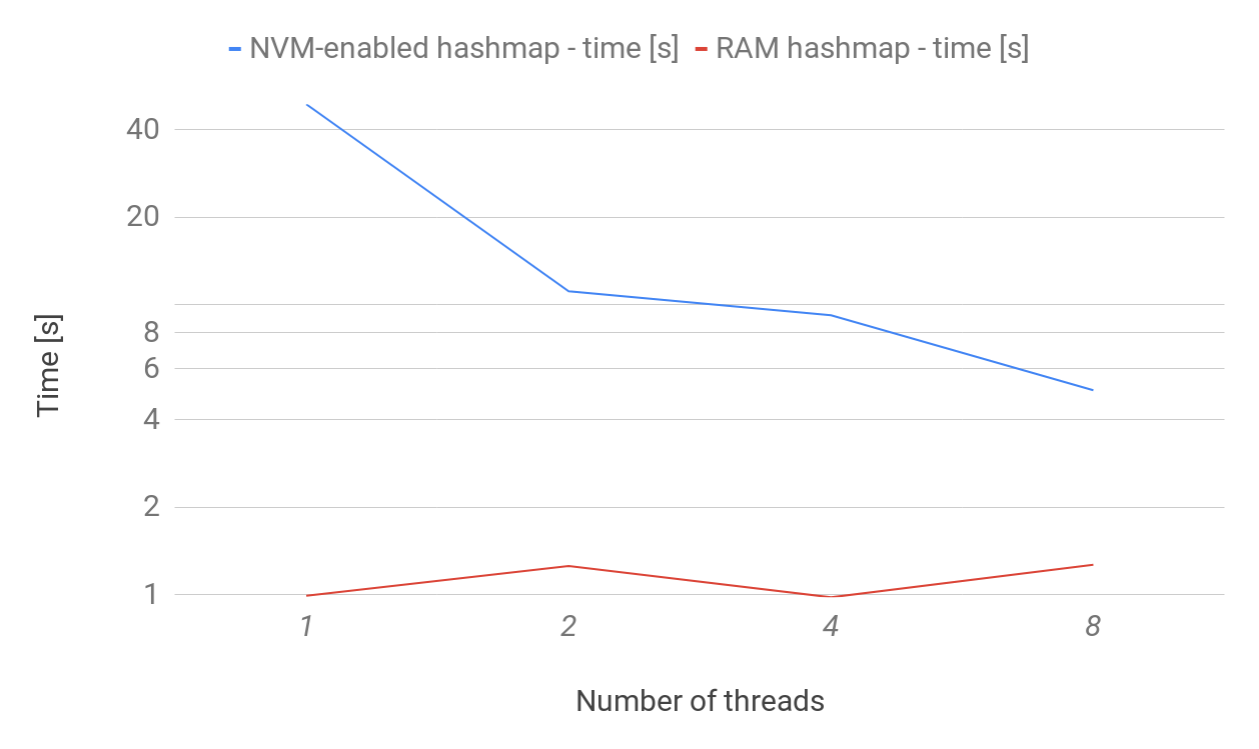
\includegraphics[width=0.8\textwidth]{thesis/figures/insert.png}
        \caption{Time measurements for \insertMethod operation comparing the NVM-enabled hashtable with unordered map}
        \label{insertPlot}
    \end{figure}
    
    \begin{figure}[ht]
        \centering
        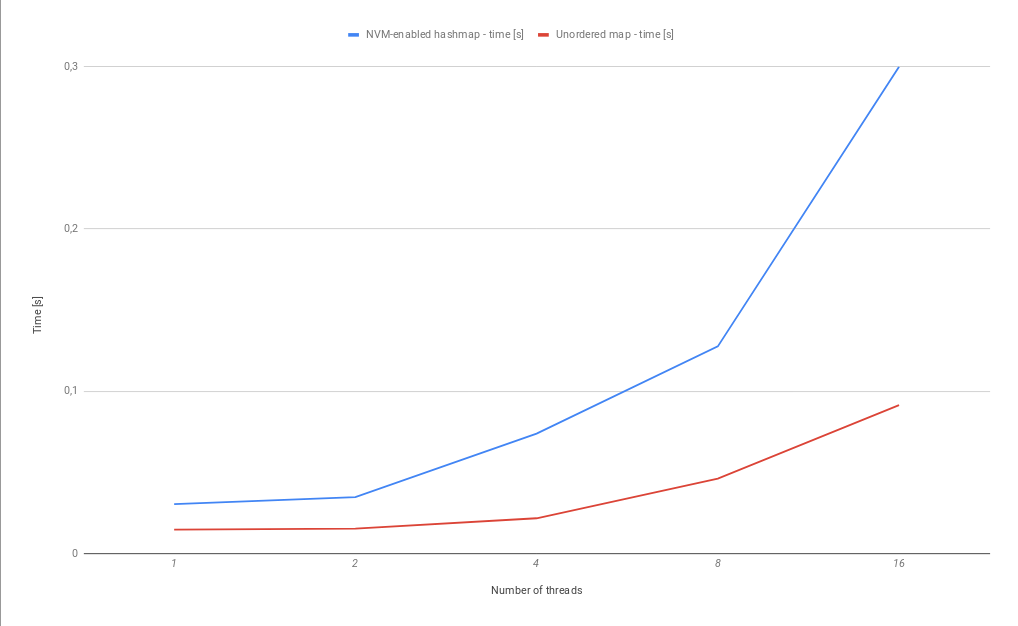
\includegraphics[width=0.8\textwidth]{thesis/figures/get.png}
        \caption{Time measurements for \getMethod operation comparing the NVM-enabled hashtable with unordered map}
        \label{getPlot}
    \end{figure}
    
    \begin{figure}[ht]
        \centering
        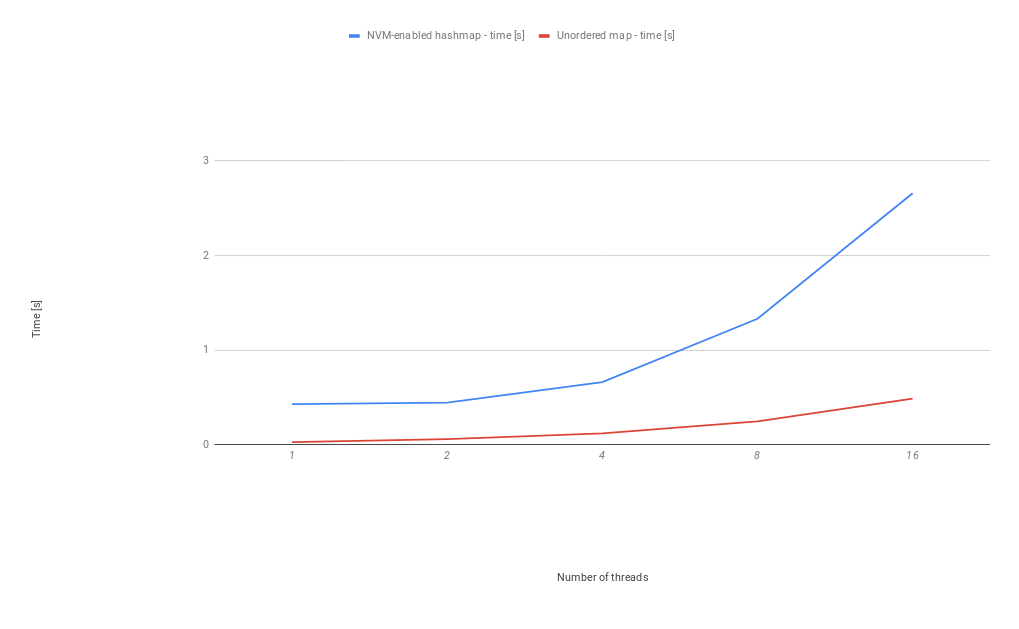
\includegraphics[width=0.8\textwidth]{thesis/figures/remove.png}
        \caption{Time measurements for \removeMethod operation comparing the NVM-enabled hashtable with unordered map}
        \label{removePlot}
    \end{figure}
    
    
    The tests results are shown on plots in Figures \ref{insertPlot}, \ref{getPlot} and \ref{removePlot}. One can see that in all test cases there is a noticeable NVM-induced time overhead, but both implementations scale similarly with the increasing number of threads. 
    
    The \getMethod method is about three times slower in the \NvmHashMap compared to the \texttt{find} method of \unorderedMap. It is due to the fact, that when using NVM, we need to \tk{maybe perform more accesses to the memory? look at the log? do you know?}
    
    Both the \insertMethod and \removeMethod operations require about five times more time to complete compared to the same operations on \unorderedMap which uses volatile RAM. The \insertMethod operation takes the longest time since it allocates memory and creates a new object. Furthermore, it requires an exclusive access to an \internalHashMap and resizes it when necessary. Since we insert \tk{how many} key-value pairs in each test, each \internalHashMap expands \tk{how many} times on average. The \removeMethod method turns out to be a little bit faster compared to the \insertMethod method, because freeing an object requires less work compared to allocating memory. Still, however, \removeMethod needs to do so in a \tk{pmdk transaction?}.
    
    All methods take more time as the number of threads increases, as a natural consequence of using locks \tk{Is this the correct reason? Remember, you have only 2 cores. It would be good to run those tests on a machine that has more cores (HPC nodes have 4).}. 
    
    \noindent \tk{What about the memory footprint? How many key-value pairs can you insert into lets say 100MB of memory in \PHT and \unorderedMap?}.
    
    To sum up, \PHT is a few times slower compared to the \unorderedMap, but it allows data to be recovered upon process crash. The observed overhead is due to additional processing required when working with NVM: \tk{maybe something like: all operations on the persistent objects are performed within transactions which means that accessing each object requires writes to the internal PMDK log? this should be explained in Section 3.2.4 }. However, both implementations scale similarly well. 
            
\section{Conclusions}
        
    In this chapter we discussed \PHT, a custom-built hash table, which supports non-volatile memory. 
    % Implementing it meant overcoming a number of challenges, e.g. correctly defining operations within \tk{pmdk?} transactions, handling generic data types in and concurrency or choosing the suitable hash function. 
    % \tk{This kind of sentence probably should be in the final conclusions.} However, using the \libpmemobj library has helped us to understand better how NVM works. 
    Extensive tests allowed us to ensure its correctness and uncover several subtle bugs related to ensuring consistency of data upon process crashes.
    
    Unsurprisingly, \PHT turns out to be slower than a standard C++ (concurrent)  implementation of a hash table, which relies solely on RAM. Our tests indicate that using NVM incurrs a significant but still acceptable overhead: the basic operations, such as the \getMethod, \insertMethod or \removeMethod methods, take about 3-5 times more time to complete compared to the corresponding operations of the standard hash table. \PHT also requires \tk{how much} more memory compared to its traditional counterpart. \PHT handles well workloads in which there are multiple threads accessing it at the same time. \PHT's scalability is on par with the scalability of the standard hash table implementation.
    
